\section{Exact audits and controlled performance measurements}
\label{sec:experiments}

The experiments answer three separate questions: whether the new
algorithm emits the complete correct ray set, whether its certificates
can be replayed independently, and whether the implementation improves
the intended stage against a relevant incumbent.  Exact output
comparisons use primitive full standard-coordinate vectors, not only
ray counts or quadrilateral supports.  Timings are secondary to these
correctness checks and do not establish an asymptotic exponent.

\subsection{Frozen complete oracle and unchanged support selection}

The principal audit reuses the preceding report's frozen discovery
corpus: 48 valid compact orientable triangulations with one torus
boundary, including solid tori, knot exteriors, and connected-sum
controls.  Its SHA-256 is
\begin{center}\footnotesize\ttfamily
0433e6c7d99bb402b79909467a7eada862ca\\
004dc4082ee25794add0e712914e
\end{center}
The driver preserves the prior support-selection rule: occupied
supports of the observed quadrilateral and standard rays, the empty
support, all supports on one or two tetrahedra, all compatible
supports for sources with at most three tetrahedra, and 64
deterministically seeded full sectors for larger sources.
Duplicate supports are removed.  This gives exactly the same 9,995
selected source/support pairs as before.  It is a finite,
oracle-informed audit design, not an unbiased input distribution or
a proposed complete sector-discovery algorithm.

One prepared source is built per triangulation.  Every eligible
sector is enumerated completely.  Its output is compared with the
frozen complete standard-coordinate vertex list restricted to that
sector, after pure links are removed.  The resulting figures are
shown in Table~\ref{tab:corpus}.  The new method covers all 9,344
previously eligible cases and 463 additional cases of raw nullity
three.  The 188 higher-nullity cases are retained as out of scope.

\begin{table}[htbp]
\centering
\caption{Complete frozen-corpus audit.  An occurrence counts a ray
again if it lies in several selected sectors.}
\label{tab:corpus}
\small
\begin{tabular}{lrr}
\toprule
Quantity & All eligible \(d\le3\) & New \(d=3\) cases\\
\midrule
Sectors & 9,807 & 463\\
Standard-ray occurrences & 7,674 & 2,821\\
Occurrences absent from Q-vertex lists & 2,279 & 1,475\\
Essential-disc occurrences & 332 & 129\\
Non-Q essential-disc occurrences & 118 & 84\\
Distinct source/ray pairs & 1,663 & 969\\
Distinct non-Q source/ray pairs & 1,046 & 759\\
Distinct essential source/ray pairs & 105 & 55\\
Distinct non-Q essential source/ray pairs & 57 & 47\\
\bottomrule
\end{tabular}
\end{table}

All 9,807 eligible ray sets agree exactly.  The non-Q counts show
why a quadrilateral-vertex oracle alone would not test the claim
being made.  The distinct-source/ray figures remove multiplicity
from repeated appearances in overlapping sectors.  They should
not be added to the occurrence counts.

\begin{table}[htbp]
\centering
\caption{Raw matching nullity and actual projective dimension.
The degenerate cases occur in genuine triangulations.}
\label{tab:strata}
\small
\begin{tabular}{rrrrrr}
\toprule
Raw \(d\) & Empty & Point & Segment & Polygon & Total\\
\midrule
0 & 5,357 & 0 & 0 & 0 & 5,357\\
1 & 890 & 1,947 & 0 & 0 & 2,837\\
2 & 29 & 140 & 981 & 0 & 1,150\\
3 & 1 & 3 & 39 & 420 & 463\\
\bottomrule
\end{tabular}
\end{table}

The dimension breakdown in Table~\ref{tab:strata} is important.
It would be incorrect to treat every raw three-dimensional kernel
as a positive-area polygon or to infer emptiness from a missing
two-dimensional interior.  Thirteen retained coverage certificates
span every observed pair of raw and feasible dimension.  A separate
replay-only process accepts all thirteen.  This does not mean
every corpus certificate was serialized and replayed: the full
audit compares every output, while independent retained replay
covers the selected dimension strata.

Eight complete standard-coordinate lists were freshly regenerated
using Regina 7.4 and matched the frozen lists: the four cap
controls with identifiers \code{cap\_1\_2\_2},
\code{cap\_1\_2\_3}, \code{cap\_3\_5\_2},
\code{cap\_3\_5\_3}; finite trefoil and figure-eight interiors;
\code{solid\_torus\_sum\_s2xs1}; and
\code{fibonacci\_lst\_10}.  Their complete lists contain
35, 83, 52, 120, 55, 446, 69, and 107 standard vertices,
respectively.  The source snapshot remained unchanged throughout
the audit.  The digest of all eligible computed output sets is
\begin{center}\footnotesize\ttfamily
3ebe4355456c91c036c5ef40b0c81361b17\\
aa92666e87a1130195421f3fa1687.
\end{center}

The largest observed sector output has seven rays, the largest
number of nontrivial active groups is two, and the largest observed
number of cross-group segment-pair tests is one.  Thus this corpus
is useful for correctness and degeneracies, but it does not
empirically realize the growing quadratic worst case.

\subsection{Additional independent and adversarial checks}

An additional differential driver compares 1,646 genuine eligible
sectors, with 2,712 ray occurrences, against the incumbent
arrangement and an independent active-rank test.  It also checks
240 abstract potential cones, containing 449 output vertices,
against an independently generated all-equalities arrangement
followed by extremality filtering.  These audits are supplementary;
their sources overlap earlier controls and their counts should
not be summed into an asserted number of distinct triangulations.

The focused suite contains 31 passing tests across the sparse
constructor, exact planar geometry, adversarial coverage replay,
and disc-search composition.  The unchanged maintained
sector-integration suite adds eight passing tests.  The focused
checks include all 64 allowed/absent type choices on a small
two-cap source; 292 exact sparse/incumbent kernel-field comparisons;
180 deterministic random rational clipping cases against an
independent halfplane-intersection oracle; abstract grids;
inactive equalities; coincident minimum edges; and raw nullity-three
cones with empty, point, and segment sections.

Coverage mutations exercise wrong sources, charts, labels, missing
and duplicated cells, reversed polygon order, shrunken sections,
missing or reordered rays, malformed rationals, Boolean values
in integer fields, and cancellation callbacks.  The checker is
also exercised with the producer disabled.  The discovery tests
replay a positive witness, replay empty and nonempty sector
exhaustion, reject incomplete per-ray disc checks, and ensure a
ray allowance cannot manufacture an exhaustion certificate.
These are targeted regression tests for material correctness
risks, not a claim of exhaustive testing of every malformed
input to all inherited repository modules.

\subsection{Geometric family verification}

The double-cap family was checked at \(n=1,2,4,8\), independently
of the timing experiment.  All 28 predicted ray vectors are
classified by both native compressed component certificates
with replay and Regina: each is a connected orientable disc
with one boundary component; four per source are essential
and three are inessential.  The audit additionally checks
300 deterministic canonical-formula grid points and twelve
mixed directions, confirming the predicted counts
\(x+h\) components and \(x\) essential discs.

Fresh complete Regina standard lists at these four sizes contain
35, 39, 85, and 375 vertices.  Restricting each complete list
to the designated sector leaves exactly seven nonlink rays.
Four further complete coverage certificates are replayed in
a separate process.  The all-\(n\) assertions in
Section~\ref{fib:family} rest on the face-equation and
topological proofs; these finite calculations check the
fixture conventions and implementation against those proofs.

\begin{figure}[htbp]
\centering
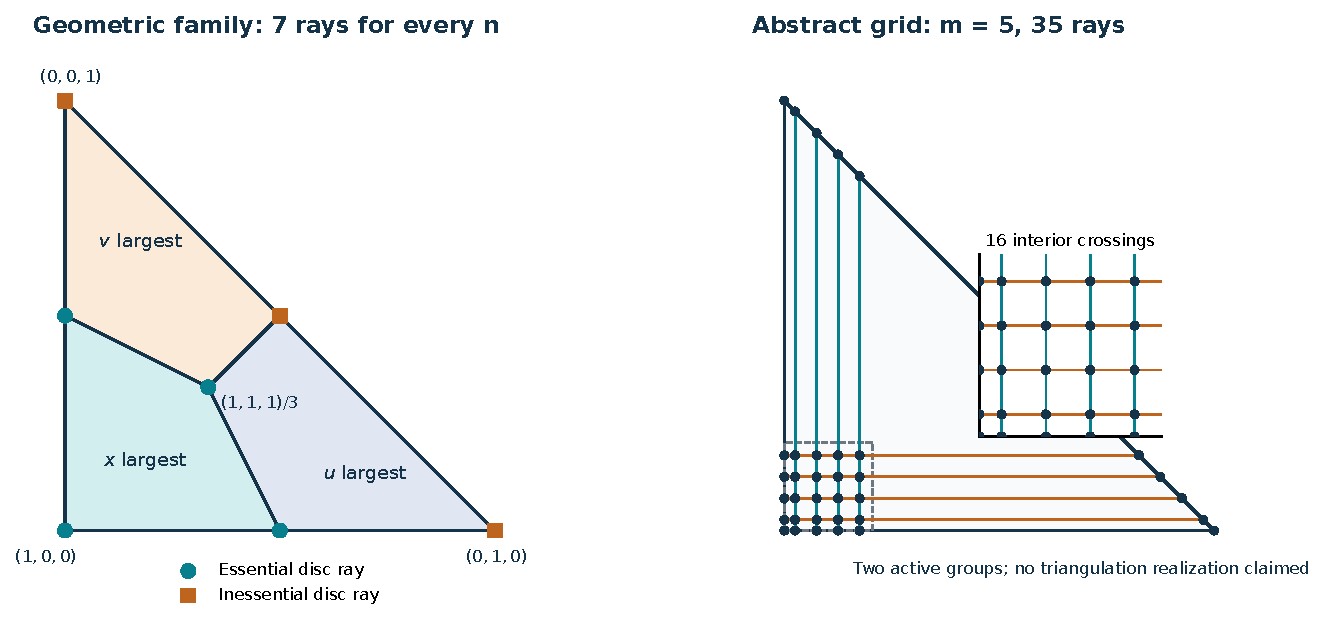
\includegraphics[width=.92\linewidth]{figures/minimum_diagrams.pdf}
\caption{Exact geometric models.  Left: the seven-vertex
two-cap diagram, drawn in the rescaled parameter section \(x+u+v=1\) with
\(u=y/A,\ v=z/A\).  Each region corresponds to the largest
of \(x,u,v\), or equivalently the active minimum after a
common affine shift.  Right: the abstract two-group grid
at \(m=5\), with \(m^2+2m=35\) vertices.  Only the left
diagram is asserted here to come from the exhibited
triangulated solid-torus family.}
\label{fig:diagrams}
\end{figure}

\subsection{Paired complete-enumeration timings}

The primary performance experiment uses \(n=1,2,4,8,16,32\)
base tetrahedra and \(t=n+2\) total tetrahedra.
For each size it retains a warmup and three paired rounds,
alternating the execution order.  The \emph{full} incumbent
arm builds the original kernel and enumerates with the
maintained automatic dispatcher; the full new arm builds
the sparse kernel and enumerates with the planar routine.
The dispatcher selects the old arrangement on this family.
Two additional arms use the \emph{same already constructed}
incumbent kernel, isolating enumeration after matching.

The timed task is complete ray-list exhaustion.  Full arms
include native geometry preparation, exact matching
construction, enumeration, and all native coordinate
checks performed during lifting.  Fixture generation,
shared-kernel setup, hashes, formula-vector comparison,
and serialization are outside the timers.  Disc-component
classification, independent coverage replay, sector
discovery, and whole-knot recognition are not timed here.
Every completed arm returns exactly the seven formula rays;
the old hyperplane, positive-direction, rejected-direction,
and pair-candidate counters match the all-size formulas.

% Generated from evidence/benchmark_summary.json; all times are milliseconds.
\begin{table}[htbp]
\centering
\small
\setlength{\tabcolsep}{3.8pt}
\begin{tabular}{r rrr rrr}
\toprule
& \multicolumn{3}{c}{Full construction and enumeration}
& \multicolumn{3}{c}{Enumeration on the same kernel} \\
\cmidrule(lr){2-4}\cmidrule(lr){5-7}
$n$ & Incumbent & Planar & Paired ratio & Incumbent & Planar & Paired ratio \\
\midrule
1 & 4.238 & 2.720 & 1.47 & 3.002 & 2.363 & 1.27 \\
2 & 8.550 & 3.057 & 2.83 & 8.224 & 2.898 & 2.84 \\
4 & 46.490 & 5.209 & 8.90 & 47.096 & 4.367 & 10.79 \\
8 & 537.411 & 8.730 & 61.64 & 530.946 & 6.916 & 73.80 \\
16 & 8\,572.669 & 19.861 & 482.82 & 8\,749.966 & 11.624 & 758.84 \\
32 & $40\,000$ cap & 48.458 & -- & $40\,000$ cap & 25.997 & -- \\
\bottomrule
\end{tabular}
\caption{Complete seven-ray enumeration for the double-capped Fibonacci family.
Times are medians of three alternating-order paired rounds, in milliseconds;
one warmup per arm is retained in the raw data and excluded from these medians.
Paired ratios are medians of within-round incumbent/planar time ratios,
not ratios of the displayed medians. For example, at $n=16$ the full paired
ratio is $482.82$, whereas the ratio of medians is $431.64$.
The two post-kernel arms receive exactly the same immutable incumbent-built kernel.
At $n=32$, all eight incumbent warmup/round runs reach the cooperative
$40\,000$\,ms cap after emitting seven rays but before proving enumeration
complete; the cap entries are allowances, not completed-run medians,
and no speed ratio is reported.}
\label{tab:planar-enumeration-benchmarks}
\end{table}

\begin{table}[htbp]
\centering
\small
\begin{tabular}{r rrrr}
\toprule
$n$ & Prior envelope (ms) & Planar (ms) & Paired prior/planar & Ratio of medians \\
\midrule
8 & 2.193 & 2.415 & 0.92 & 0.91 \\
32 & 8.534 & 8.741 & 0.97 & 0.98 \\
\bottomrule
\end{tabular}
\caption{Control against the earlier optimized nullity-two envelope enumerator,
loaded unmodified from the preceding research package. Both arms use the same
incumbent-built kernel and return the same three formula rays. Times are
medians of three paired rounds; values below one in either ratio column
indicate a slower planar implementation. These controls show no measured
advantage over the already optimized nullity-two method.}
\label{tab:planar-prior-envelope-control}
\end{table}

\begin{table}[htbp]
\centering
\small
\setlength{\tabcolsep}{4pt}
\begin{tabular}{r rrr rr}
\toprule
& \multicolumn{3}{c}{Complete construction (ms)}
& \multicolumn{2}{c}{Paired incumbent/sparse ratios} \\
\cmidrule(lr){2-4}\cmidrule(lr){5-6}
$k$ & Incumbent & Sparse once & Sparse reused & Reused source & Both cached \\
\midrule
1 & 72.133 & 81.463 & 8.004 & 8.84 & 1.88 \\
8 & 44.435 & 51.755 & 5.638 & 7.88 & 2.06 \\
32 & 61.126 & 64.297 & 12.041 & 4.74 & 2.02 \\
\bottomrule
\end{tabular}
\caption{Separate sparse-constructor measurements on supplied sparse sectors
of $t=1024$ layered solid tori. Times are medians of five paired rounds and
include unchanged exact rational elimination. The reused-source column
excludes its one-time preparation, while both ordinary single-call
constructors include preparation. The last column uses an additional control
where both constructors receive already validated geometry; it isolates
sparse kernel construction from validation reuse. Ratios are medians of
within-round ratios. The single-call sparse constructor is slower on these
cases. These are construction measurements, separate from complete ray
enumeration and from whole-knot recognition. All nine constructor cases
and every raw sample are retained in the data files.}
\label{tab:planar-sparse-source-control}
\end{table}


The \(n=32\) incumbent hits the cooperative 40-second
completion limit in both warmups and all six timed
incumbent rounds.  It has already emitted seven genuine
rays, but has not finished eliminating the other candidate
directions.  Its records are resource-limited, and no
speedup ratio is assigned to that size.  This is precisely
why the benchmark does not measure merely the time to
observe seven answers or the time to the first positive
disc.  A cooperative cap can overshoot by the duration
of an indivisible exact operation.

The rank-two control loads the preceding optimized
\code{sector\_envelope.py} unchanged and compares it with
the new method on the same kernel.  The older specialized
method is slightly faster in these measurements.  This
negative result argues for preserving the earlier branch
when designing an eventual dispatcher.  It would be
misleading to claim improvement over that method by
comparing only with an older all-equalities implementation.

\begin{figure}[htbp]
\centering
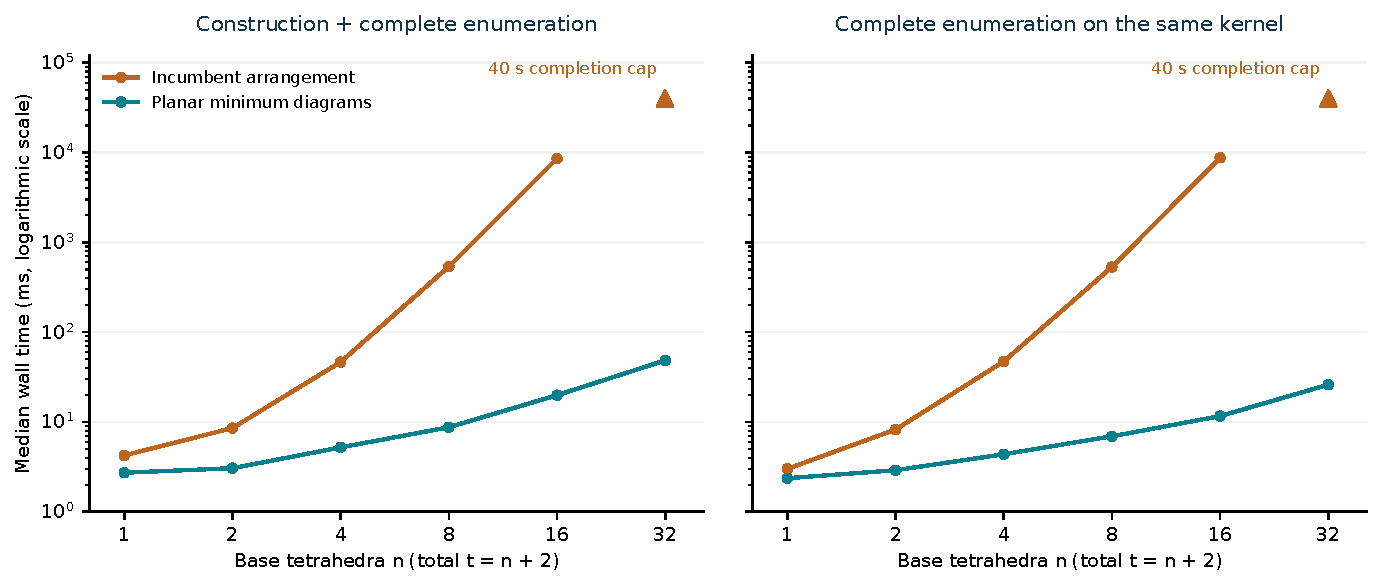
\includegraphics[width=.92\linewidth]{figures/paired_times.pdf}
\caption{Median complete-enumeration wall time over three
paired rounds, with logarithmic axes.  The incumbent
\(n=32\) value is a resource limit, displayed as a cap
marker rather than a completed timing.  These are
stage measurements on one growing family, not a fitted
worst-case exponent or a whole-recognizer speedup.}
\label{fig:times}
\end{figure}

\subsection{Construction-only reuse controls}

The separate sparse-constructor experiment uses nine
supplied-support cases on growing layered solid tori
and five rounds per case.  It distinguishes original
complete construction, one-shot sparse construction,
reused sparse construction, and a control in which
both constructors receive reusable prepared geometry.
Using ratios of median times across these cases, reused sparse construction is
1.38--9.01 times as fast as original complete construction.
When both reuse geometry, the measured ratio is
1.10--2.14.  One-shot sparse construction gives ratios
0.76--0.99 and is slower in this sample.

At \(t=1024,k=32\), original complete construction has
median 61.126 ms, one-shot sparse construction 64.297 ms,
and reused sparse construction 12.041 ms.  The matched
prepared-geometry control is 27.334 ms for the old builder
and 12.802 ms for the sparse builder.  Dense label entries
fall from 196,512 to 4,032.  This gives a concrete allocation
explanation while exposing the cost of preparing a
source that will be used only once.

All reported timings are observations from Python 3.12.14
in the supplied execution environment.  Exact source
digests, raw wall and CPU times where recorded, execution
order, counters, caps, and output hashes accompany the
package.  Three or five rounds on selected sources do
not support confidence claims about unrelated hardware
or a general input distribution.
